\section{Methodology}
\label{sec:method}

We present \cubic, a curvature-driven dynamic caching framework for FM generation. The core idea is to connect local trajectory geometry with runtime caching decisions: regions whose trajectories are locally straighter can tolerate more aggressive cache reuse, whereas regions with higher curvature should be refreshed more frequently. 


\subsection{Overview of the Inference Pipeline}
\label{sec:method_overview}

As illustrated in Fig.~\ref{fig:overview}, \cubic exploits the spatial heterogeneity of permissible step sizes by transforming the standard ODE solving process into an \emph{anchor-selective inference loop}. 

\begin{figure}[t]
    \centering
    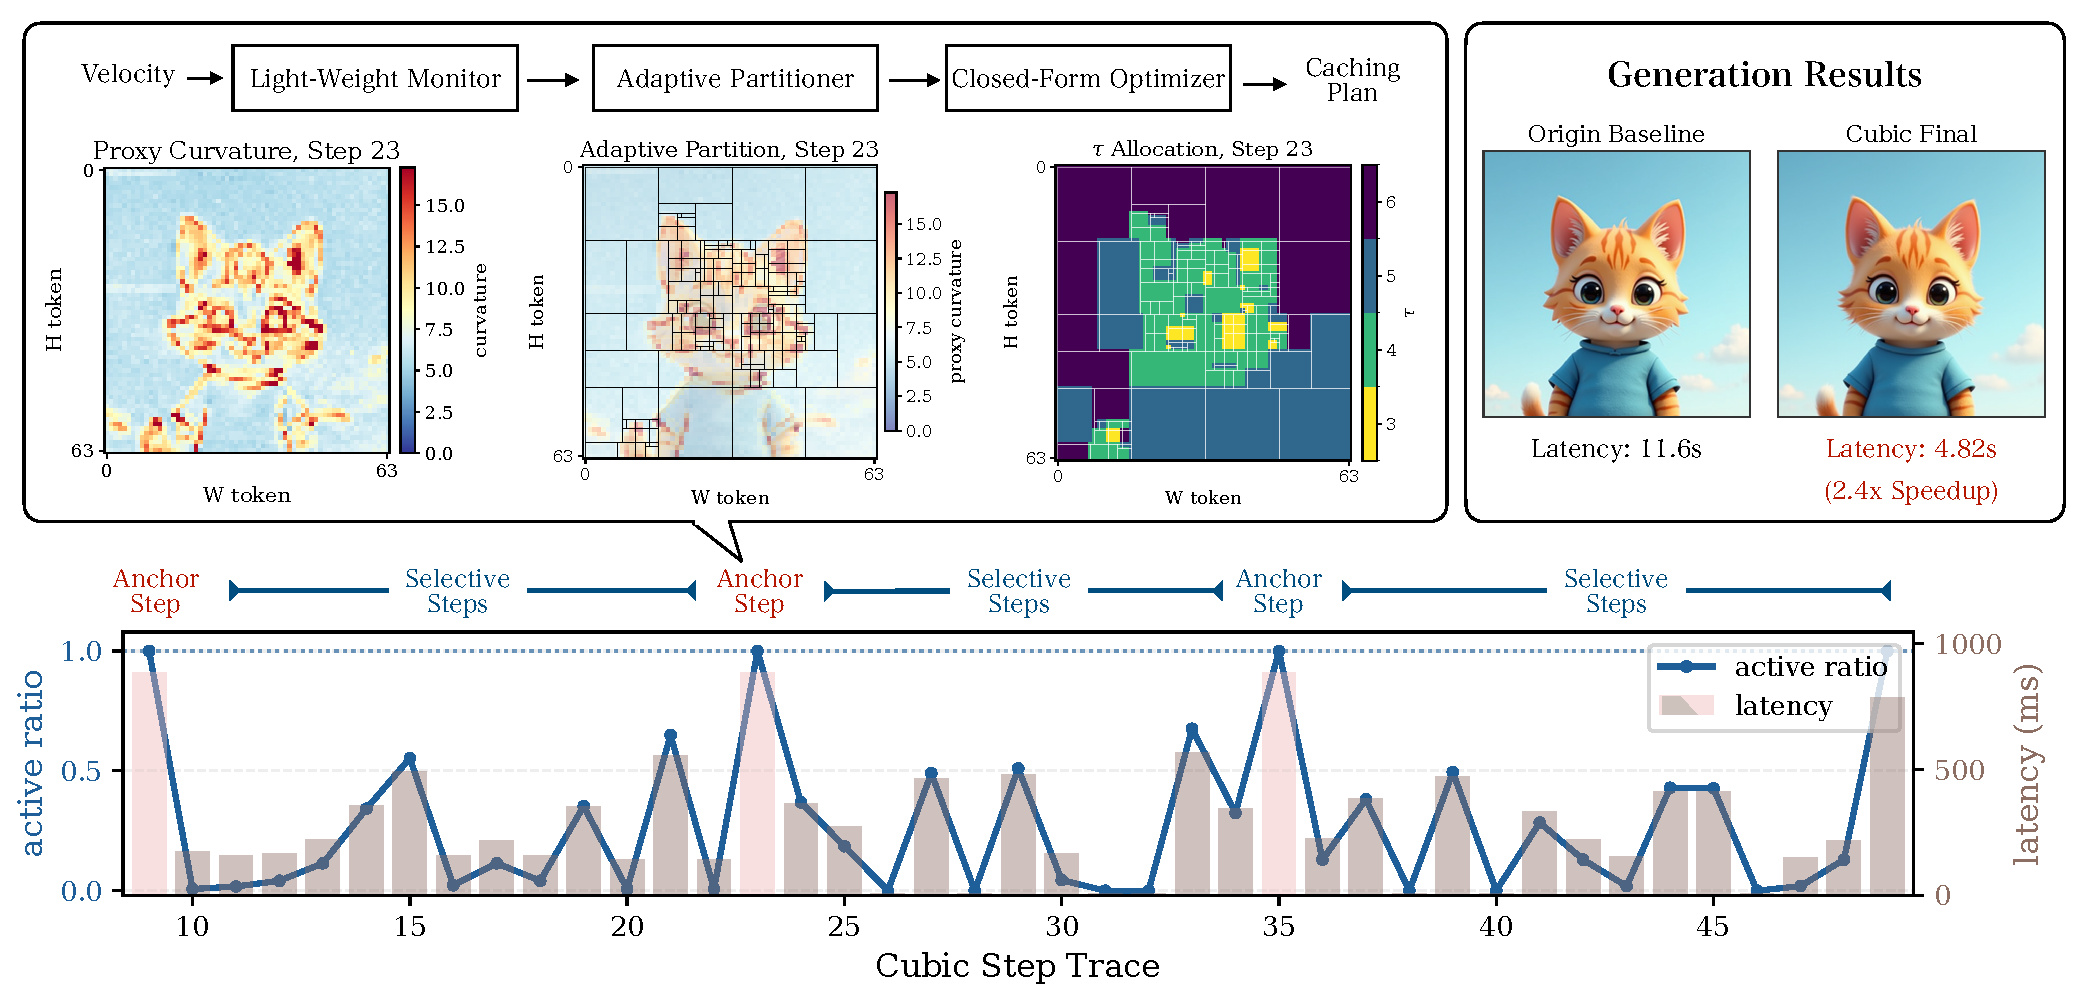
\includegraphics[width=\linewidth]{figure/overview.pdf}
    \caption{\cubic overview.}
    \label{fig:overview}
\end{figure}

The pipeline alternates between two types of steps:
\begin{itemize}
    \item \textbf{Anchor Steps:} Full forward passes that act as the ``brain'' of the system. They refresh the exact velocity prediction for all tokens, measure the geometric properties of the trajectory, and dynamically re-evaluate the caching policy.
    \item \textbf{Selective Steps:} Sparse forward passes that act as the ``muscle'' for acceleration. They compute only a dynamically chosen subset of tokens (active tokens), while the remaining tokens (frozen tokens) reuse cached intermediate states.
\end{itemize}
This anchor-selective decoupling divides the acceleration mechanism into two clean phases: \emph{estimation \& optimization} at anchor steps (Sec.~\ref{sec:anchor_step}), and \emph{sparse execution} at selective steps (Sec.~\ref{sec:selective_step}).
The two phases rest on different kinds of justification. The curvature proxy, the error model, and the budget-constrained interval allocation are derived from the ODE analysis in Appendix~\ref{app:cubic_theory}. The anchor horizon and the block partition are empirical system choices: they do not change the allocation rule, but select an operating point on the latency--quality frontier for a given architecture (Appendix~\ref{app:extra_exp}).
% This pipeline turns local trajectory geometry into a concrete execution policy: the monitor estimates curvature, the partitioner designs granularity, the optimizer assigns refresh intervals, and the runtime engine realizes those decisions as selective token computation.


\subsection{Anchor Steps: Estimation and Optimization}
\label{sec:anchor_step}

\paragraph{Curvature Estimation}
Directly computing local trajectory curvature is impractical at inference time because it requires Jacobian information which is expensive to compute. We therefore seek an online proxy that introduces light weight system cost. Our key observation is that if a token trajectory is locally straight, then its endpoint predicted by the current velocity field should remain nearly unchanged across successive observations. In contrast, trajectory curvature causes this endpoint prediction to drift.

For a spatial token indexed by $i$, we define its endpoint prediction at time $t$ as
\begin{equation}
    \hat{x}_1^{(i)}(t) = x^{(i)}(t) + (1 - t)\, v_\theta^{(i)}(x(t), t).
\end{equation}
Importantly, the monitor is updated only at anchor steps rather than at every sampler step. Let $\{t_{a_m}\}_{m=1}^{M}$ denote the anchor-step sequence. Interpreted in Fig.~\ref{fig:method}, we define the endpoint prediction drift between two consecutive anchor observations as
\begin{equation}
    \hat{\delta}^{(i,m)} = \hat{x}_1^{(i)}(t_{a_m}) - \hat{x}_1^{(i)}(t_{a_{m-1}}).
\end{equation}
As derived in Appendix~\ref{app:curvature_proxy}, to first order this drift scales proportionally to the local trajectory curvature $\kappa^{(i)}(t_{a_m})$, modulated by the remaining time horizon $(1-t_{a_m})$ and the step interval $\Delta t_{a_m} = |t_{a_m} - t_{a_{m-1}}|$.

Rearranging this relation directly gives the online curvature estimate:
\begin{equation}
    \hat{\kappa}^{(i)} = \left\|\hat{\delta}^{(i,m)}\right\|/\left[(1-t_{a_m})\,\Delta t_{a_m}\right].
\end{equation}

In practice, we compute this proxy in latent space and aggregate it to the token grid using the same patch granularity as the underlying DiT tokenizer, producing a token-space curvature map $\kappa \in \mathbb{R}^{F_t \times H_t \times W_t}.$ 

% \paragraph{Dynamic Spatial Partitioning}
% Assigning independent caching intervals to individual tokens incurs prohibitive scheduling overhead. Instead, \cubic groups adjacent tokens into rectangular blocks $\{B_b\}$ with shared update intervals. Crucially, to match the granularity to local trajectory complexity—fine blocks for curved regions, coarse blocks for straight regions—the partitioning must be spatially adaptive.

% Derived in Appendix~\ref{app:parition}, rather than relying on fixed grids, \cubic extracts a continuous geometric prior directly from the curvature map to guide the partitioning. We first isolate high-curvature "foreground" regions via thresholding and stabilize their boundaries. Using this prior, we then recursively bisect the token grid: foreground-dominated regions are assigned a finer target granularity, while background-dominated regions are assigned a coarser target. A region is split only if it exhibits mixed complexity (high intra-region variance) or exceeds its assigned target dimensions. 

% This yields adaptively-sized, strictly rectangular blocks that naturally conform to the underlying image geometry. Because this adaptive partitioning inherently isolates high-curvature outliers into dedicated finer blocks, we can safely represent each block's risk using a simple spatial mean:
% \begin{equation}
%     \kappa_b = \frac{1}{|B_b|} \sum_{i \in B_b} \hat{\kappa}^{(i)}.
% \end{equation}
% This block-wise curvature map $\{\kappa_b\}$ serves as the direct input for the subsequent budget-constrained interval optimization.

However, assigning independent caching intervals to individual tokens incurs prohibitive scheduling overhead. Instead, \cubic groups adjacent tokens into rectangular blocks $\{B_b\}$ that share a unified update interval. Sharing an interval also keeps neighboring tokens, which attend to each other with high attention weights in DiT self-attention, at the same cache age. Under per-token schedules, adjacent tokens would read keys and values computed at different steps (Sec.~\ref{sec:selective_step}), and this local inconsistency propagates through subsequent layers. To balance spatial granularity and scheduling efficiency, we employ a lightweight partitioning strategy guided by the curvature map (detailed in Appendix~\ref{app:parition}). Once the partition $\mathcal{P}=\{B_b\}$ is established, we aggregate the token-wise proxy into a representative block-wise score using a spatial mean:
    $\kappa_b = \frac{1}{|B_b|} \sum_{i \in B_b} \hat{\kappa}^{(i)}.$
This block-wise curvature map $\{\kappa_b\}$ serves as the direct input for the subsequent budget-constrained interval optimization.

\paragraph{Cache Error Modeling}
After obtaining a representative curvature for each block, \cubic determines how long each block may safely reuse cached outputs. Consider a block $b$ that is fully recomputed at an anchor step $t_0$, yielding the cached velocity $v_{\text{cache}}^{(b)} = v_\theta^{(b)}(x(t_0), t_0)$. If this block is frozen for the subsequent $\tau_b$ selective steps, the same cached velocity is continuously reused throughout the interval $[t_0, t_0+\tau_b \Delta t]$.

Let $x_{\text{exact}}^{(b)}(t)$ denote the exact trajectory, and $x_{\text{cache}}^{(b)}(t)$ denote the trajectory obtained by reusing the cached velocity. We define the cache-induced state truncation error at the end of the reuse window as:
\begin{equation}
    \varepsilon_{\tau_b}^{(b)} = x_{\text{cache}}^{(b)}(t_0 + \tau_b \Delta t) - x_{\text{exact}}^{(b)}(t_0 + \tau_b \Delta t).
    \label{eq:error_def}
\end{equation}
As derived in Appendix~\ref{app:error_modeling}, if the curvature is bounded within the reuse window, this accumulated error is bounded by the local trajectory curvature:
\begin{equation}
    \label{eq:error_bound}
    \left\|\varepsilon_{\tau_b}^{(b)}\right\|
    \lesssim
    \frac{1}{2}\,\kappa_b\,\tau_b^2\,\Delta t^2.
\end{equation}
This result directly exposes the desired behavior: blocks with low curvature can tolerate longer reuse intervals, while high-curvature blocks should be updated more often.

\paragraph{Update Interval Optimization} 
\label{sec:optimizer}

We formalize interval allocation as a budget-constrained optimization problem. Let $\rho$ denote the target speedup, $\tau_b$ the update interval for block $b$, and $|\mathcal{B}_b|$ its spatial size (i.e., number of tokens). Because the adaptive partitioner yields blocks of varying sizes, the optimization must be weighted by block size.

\begin{equation}
\min_{\tau_b \ge 1} \; \sum_{b=1}^{\mathcal{B}} |\mathcal{B}_b| \, \kappa_b^\alpha \tau_b^\beta
\quad \text{s.t.} \quad
\sum_{b=1}^{\mathcal{B}} \frac{|\mathcal{B}_b|}{N} \frac{1}{\tau_b} = \frac{1}{\rho},
\end{equation}
where $N = \sum_{b=1}^{\mathcal{B}} |\mathcal{B}_b|$ is the total number of tokens in the image, $\rho > 1$ is the target speedup factor, and $\tau_b \ge 1$ are the block-wise update intervals. The objective function minimizes the total expected squared error across the entire image, weighted by the number of tokens $|\mathcal{B}_b|$ per block, with the error bound per block squaring to $\kappa_b^\alpha \tau_b^\beta$. The constraint ensures that the token-weighted average update rate $\mathbb{E}[1/\tau_b]$ equals the reciprocal of the target speedup $1/\rho$, exactly enforcing the compute budget.
Note that $\rho$ specifies the compute budget of the selective steps only. Anchor steps and the full-compute steps at the beginning and end of sampling process all tokens. With $K_{\mathrm{full}}$ full-compute steps and $K_{\mathrm{sel}}$ selective steps, the overall token-compute fraction is $(K_{\mathrm{full}} + K_{\mathrm{sel}}/\rho)/(K_{\mathrm{full}} + K_{\mathrm{sel}})$, and the measured wall-clock speedup additionally reflects system overhead.
% To minimize the total expected squared error across the \emph{entire} image, the objective function is naturally weighted by the number of tokens in each block. By squaring the truncation error bound in Eq.~\ref{eq:error_bound}, we have:
% \begin{equation}
%     \min_{\tau_b \ge 1}\; \sum_{b=1}^{\mathcal{B}} |\mathcal{B}_b| \, \kappa_b^\alpha \tau_b^\beta.
% \end{equation}
% The compute budget constraint requires that the block-weighted average update rate strictly equals the reciprocal of the target speedup. Let $N = \sum_{b=1}^{B} |B_b|$ be the total number of tokens. The constraint is formulated as:
% \begin{equation}
%     \sum_{b=1}^{\mathcal{B}} \frac{|\mathcal{B}_b|}{N} \frac{1}{\tau_b} = \frac{1}{\rho}.
% \end{equation}
Intuitively, this ensures proportional FLOP savings: freezing a large block (high $|\mathcal{B}_b|$) for $\tau_b$ steps yields strictly greater computational reduction than freezing a smaller block with the same interval.

As derived in Appendix~\ref{app:optimal_interval} via the Lagrange multiplier method, the block size weights $|\mathcal{B}_b|$ appear on both the objective and the constraint. Consequently, they cancel out during the first-order optimality condition. The resulting optimum is $\tau_b^\star \propto \kappa_b^{-\gamma}$ with $\gamma=\alpha/(\beta+1)$, so the allocation depends on the two error exponents only through $\gamma$. Substituting the theoretical defaults $(\alpha,\beta)=(2,4)$ gives $\gamma=2/5$ and yields the final allocation rule:
% \begin{equation}
%     \tau_b^\star \propto \kappa_b^{-\alpha/(\beta+1)}.
% \end{equation}

\begin{equation}
    \tau_b^\star \propto \kappa_b^{-2/5}.
\end{equation}
Thus, \cubic naturally assigns shorter intervals to high-curvature blocks and longer intervals to low-curvature ones, irrespective of their spatial sizes. In implementation, the continuous solution is discretized to valid integer bounds. 

\paragraph{Effective ODE Strides}
To ensure optimized intervals translate into actual FLOP savings, anchor steps dictate a selective phase length of $2\tau_{\max}$, where $\tau_{\max} = \max_{b \in \mathcal{P}} \tau_b$. This receding-horizon rule is tied to the current allocation: it gives the blocks assigned the longest interval enough steps to execute their reuse schedule before curvature is re-estimated, so that caching operations serve as \emph{effective ODE strides} rather than being overwritten by the next anchor step. The factor of two is an empirical default rather than a theoretical optimum. If the curvature of a block changes within the window, its schedule is stale only until the next anchor step, which re-measures curvature and assigns shorter intervals to blocks whose curvature has increased. Appendix~\ref{app:anchor_ablation} compares this rule with shorter and longer horizons and with a fixed anchor gap.


\subsection{Selective Steps: Sparse DiT Execution}
\label{sec:selective_step}

% \paragraph{Anchor Step Trigger} The duration of the selective phase is dynamically determined to guarantee actual computational efficiency. Rather than using a fixed length, \cubic sets the selective phase length to $2\tau_{\max}$, where $\tau_{\max} = \max_{b \in \mathcal{P}} \tau_b$. This design ensures that even the block with the longest assigned interval completes at least one full cache reuse cycle before the global cache is refreshed at the next anchor step. Consequently, it prevents degenerate scheduling where anchor steps are triggered too frequently, which would otherwise nullify the FLOP savings of the selective phase.



\paragraph{Sparse Forward with KV Cache} Given the partition $\mathcal{P}$ and the block intervals $\{\tau_b\}$ at anchor step, the active blocks at selective step $k$ are defined as
\begin{equation}
    \mathcal{A}_k = \{ b \in \mathcal{P} \mid s_k \bmod \tau_b = 0 \},
\end{equation}
where $s_k$ is the local step index within the selective phase. The interval $\tau_b$ is an integer with $\tau_b \ge 1$. A block with $\tau_b = 1$ is recomputed at every selective step, and a block with $\tau_b > 1$ is recomputed every $\tau_b$ steps and stays frozen in between. This update-and-reuse cycle repeats until the next anchor step. The active blocks induce the active and frozen token sets
\begin{equation}
    \Omega_k^{\mathrm{act}} = \bigcup_{b \in \mathcal{A}_k} \mathcal{B}_b,
    \qquad
    \Omega_k^{\mathrm{frz}} = \Omega \setminus \Omega_k^{\mathrm{act}}.
\end{equation}

At each DiT layer, \cubic only computes the active tokens. To maintain full-sequence spatial dependencies without recomputing frozen tokens, the attention mechanism for active tokens queries against a reconstructed full sequence. Specifically, the newly computed Key/Value (KV) tensors for active tokens are concatenated with the cached KV tensors of frozen tokens to form the full KV states:
\begin{equation}
    K_\ell^{\mathrm{full}} = K_\ell^{\mathrm{act}} \oplus K_\ell^{\mathrm{frz}}, \quad
    V_\ell^{\mathrm{full}} = V_\ell^{\mathrm{act}} \oplus V_\ell^{\mathrm{frz}}.
\end{equation}
Attention is then evaluated as:
\begin{equation}
    Y_\ell^{\mathrm{act}} =
    \mathrm{Attn}\!\left(
    Q_\ell^{\mathrm{act}},
    K_\ell^{\mathrm{full}},
    V_\ell^{\mathrm{full}}
    \right).
\end{equation}
Crucially, after the attention computation, \cubic updates the cached KV entries for the active tokens in-place with the newly computed $K_\ell^{\mathrm{act}}$ and $V_\ell^{\mathrm{act}}$. This ensures that the per-layer KV cache progressively incorporates the latest cross-token interactions across successive steps, rather than remaining strictly static. The final output of the selective step is then formed by merging newly computed active-token outputs with cached frozen-token outputs.
% \begin{equation}
%     v_k(\Omega) =
%     \mathrm{Merge}\!\left(
%         v_k^{\mathrm{act}}(\Omega_k^{\mathrm{act}}),
%         v_{k-1,\mathrm{cache}}(\Omega_k^{\mathrm{frz}})
%     \right).
% \end{equation}

This selective forward engine is the component that actually yields computational savings: active tokens traverse the full DiT computation path, whereas frozen tokens participate only through cache reuse.

